% Digital Logic Report Template
% Created: 2020-01-10, John Miller

%==========================================================
%=========== Document Setup  ==============================

% Formatting defined by class file
\documentclass[11pt]{article}

% ---- Document formatting ----
\usepackage[margin=1in]{geometry}	% Narrower margins
\usepackage{booktabs}				% Nice formatting of tables
\usepackage{graphicx}				% Ability to include graphics

%\setlength\parindent{0pt}	% Do not indent first line of paragraphs 
\usepackage[parfill]{parskip}		% Line space b/w paragraphs
%	parfill option prevents last line of pgrph from being fully justified

% Parskip package adds too much space around titles, fix with this
\RequirePackage{titlesec}
\titlespacing\section{0pt}{8pt plus 4pt minus 2pt}{3pt plus 2pt minus 2pt}
\titlespacing\subsection{0pt}{4pt plus 4pt minus 2pt}{-2pt plus 2pt minus 2pt}
\titlespacing\subsubsection{0pt}{2pt plus 4pt minus 2pt}{-6pt plus 2pt minus 2pt}

% ---- Hyperlinks ----
\usepackage[colorlinks=true,urlcolor=blue]{hyperref}	% For URL's. Automatically links internal references.

% ---- Code listings ----
\usepackage{listings} 					% Nice code layout and inclusion
\usepackage[usenames,dvipsnames]{xcolor}	% Colors (needs to be defined before using colors)

% Define custom colors for listings
\definecolor{listinggray}{gray}{0.98}		% Listings background color
\definecolor{rulegray}{gray}{0.7}			% Listings rule/frame color

% Style for Verilog
\lstdefinestyle{Verilog}{
	language=Verilog,					% Verilog
	backgroundcolor=\color{listinggray},	% light gray background
	rulecolor=\color{blue}, 			% blue frame lines
	frame=tb,							% lines above & below
	linewidth=\columnwidth, 			% set line width
	basicstyle=\small\ttfamily,	% basic font style that is used for the code	
	breaklines=true, 					% allow breaking across columns/pages
	tabsize=3,							% set tab size
	commentstyle=\color{gray},	% comments in italic 
	stringstyle=\upshape,				% strings are printed in normal font
	showspaces=false,					% don't underscore spaces
}

% How to use: \Verilog[listing_options]{file}
\newcommand{\Verilog}[2][]{%
	\lstinputlisting[style=Verilog,#1]{#2}
}




%======================================================
%=========== Body  ====================================
\begin{document}

\title{ELC 2137 Lab 11: FSM: Guessing Game}
\author{Ashlie Lackey}

\maketitle


\section*{Summary}
This lab sought the construction of a finite state machine, FSM, to handle an irregular input from a user. We designed a synchronous FSM using ideas from both Mealy and Moore machines to create a guessing game. By first understanding how to "debounce" signals that may have an irregular input, the first step is taken to create an FSM. By the end of the experiment, participants have the skills to explain the role of finite state machines in digital systems design,ˆexplain the difference between a Mealy output and a Moore output,ˆand implement a state machine in Verilog.

\section*{Q\&A}
\begin{enumerate}
  \item At what time in the simulation did the debounce circuit reach each of the four states(zero, wait1, one, wait0)?
  
  
  \item Why can this game not be implemented with regular sequential logic?
  
  This game cannot be implemented with regular sequential logic because the input from the user is going to be irregular, and regular sequential logic cannot handle this. Therefore, an FSM is used to handle the irregular, non-repeating input that can be expected from the user.
  
  \item What type of outputs did you use for your design(Mealy or Moore)? Explain.
  

\end{enumerate}

\section*{Results}
  
Expected results table, simulation waveforms, and schematic drawings are included in this portion of the report.

\subsection*{Game Play Results on Two Settings}
Fast:(20\%)

Slow: (40\%)

\subsection*{Expected results tables}

\begin{table*}[ht]\centering
	\caption{\textit{debounce} expected results table}
	\label{ALU:tbl:alu_ERT}\medskip
	\begin{tabular}{l|rrrrrrrrrrrrrrr}
		Time (ns): & 0-5 & 5-15 & 15-40 & 40-60 & 60-80 & 80-100 & 100-120 & 120-140 & 140-160 & 160-180 & 180-200 & 200-235 & 235-245 & 245-440\\
		\midrule
		clk & 0  & 1 & 1 & 0 & 1 & 0 & 1 & 0 & 1 & 0 & 1 & ... \\
		rst & 0 & 0 & 0 & 1 & 0 & 1 & 0 & 1 & 0 & 1 & 0 & ...\\
		in & 0 & 0 & 1& 0 & 0 & 0 & 0 & 0 & 0 & 0 & 0 & ... \\
		\midrule
		out & X & X & 0 & 0  & 1 & 1 & 2 & 2 & 3 & 3 & 0 & ... \\
		tick & X & X & 0 & 0 & 0 & 0 & 0 & 0 & 1 & 1 & 0& ... \\
		\bottomrule
	\end{tabular}
\end{table*}

\begin{table*}[ht]\centering
	\caption{\textit{guess\_FSM} expected results table}
	\label{ALU:tbl:alu_ERT}\medskip
	\begin{tabular}{l|rrrrrrrrrrrrr}
		Time (ns): & 0-5 & 5-7 & 7-10 & 10-15 & 15-20 & 20-25 & 25-30 & 30-35 & 35-40 & 40-45 & 45-50 &...\\
		\midrule
		clk & 0  & 1 & 1 & 0 & 1 & 0 & 1 & 0 & 1 & 0 & 1 & ... \\
		en & 0 & 0 & 0 & 1 & 0 & 1 & 0 & 1 & 0 & 1 & 0 & ...\\
		rst & 0 & 0 & 1& 0 & 0 & 0 & 0 & 0 & 0 & 0 & 0 & ... \\
		\midrule
		count & X & X & 0 & 0  & 1 & 1 & 2 & 2 & 3 & 3 & 0 & ... \\
		tick & X & X & 0 & 0 & 0 & 0 & 0 & 0 & 1 & 1 & 0& ... \\
		\bottomrule
	\end{tabular}
\end{table*}

\begin{table*}[ht]\centering
	\caption{\textit{ggame\_test} expected results table}
	\label{ALU:tbl:alu_ERT}\medskip
	\begin{tabular}{l|rrrrrrr}
		Time (ns): & 0-2 & 2-5 & 5-10 & ... & 1000005-2000000 & 2000000-2621435 & 2621435-3000005\\
		\midrule
		data(hex) & 1234 & 1234 123 && ... & 1234  & 1234 & 1234  \\
		hex\_dec & 0 & 0 & 0 & ... & 1 &  0 & 0\\
		sign & 0 & 0 & 0 & ... & 0 &  1 & 1 \\
		reset & 0 & 1 & 0 & ... & 0 & 0 & 0  \\
		clock & 0 & 0 & 5 & ...  \\
		\midrule
		seg (hex) & X & 19 & 19 & ... & 19 & 19 & 30 \\
		dp & 1 & 1 & 1 & ... & 1 & 1 & 1 \\
		an (hex)& X & e & e & ... & e & e & d \\
		\bottomrule
	\end{tabular}
\end{table*}

\clearpage
 
\subsection*{Simulation Waveforms}
\begin{figure}[ht]\centering
	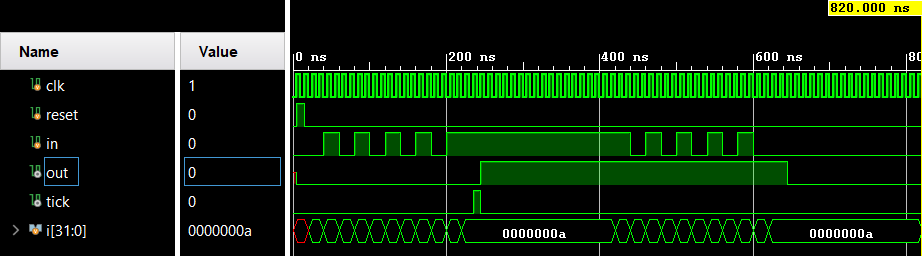
\includegraphics[width=1.1\textwidth]{debouncetest}
	\caption{\textit{debounce testbench} Simulation Waveform}
	\label{fig:sim_with_table}
\end{figure}

\begin{figure}[ht]\centering
	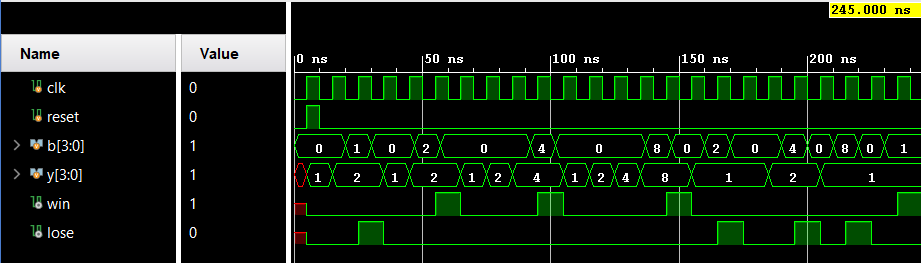
\includegraphics[width=1.1\textwidth]{gsfmtest}
	\caption{\textit{guess\_FSM testbench} Simulation Waveform}
	\label{fig:sim_with_table}
\end{figure}

\begin{figure}[ht]\centering
	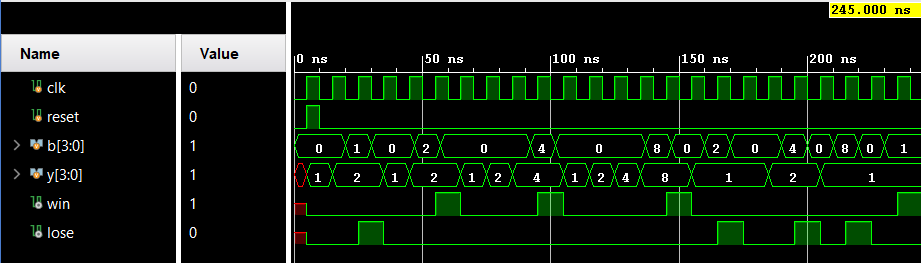
\includegraphics[width=1.1\textwidth]{gsfmtest}
	\caption{\textit{guessing\_game testbench} Simulation Waveform}
	\label{fig:sim_with_table}
\end{figure}

\clearpage

\section*{Code}
.

\begin{lstlisting}[style=Verilog,caption=guess\_FSM Verilog Code,label=code:ex ]
`timescale 1ns / 1ps
// ELC 2137,  Ashlie Lackey, 2020 -04 -21
module guess_FSM#(parameter N = 21)(input clk, reset,
	input reg [3:0] b,
	output reg [3:0] y,
	output reg win,
	output reg lose
	);
	
	localparam [2:0]
		s0 = 3'b000,
		s1 = 3'b001,
		s2 = 3'b010,
		s3 = 3'b011,
		swin = 3'b100,
		slose = 3'b101;
	
	reg [2:0] state, state_next;
	
	always_ff @(posedge clk or posedge reset)
		if(reset) begin
			state <= s0;
		end
		else begin
			state <= state_next;
	end
		
		always_comb  begin
		//  default  behavior
		state_next = state;
		//y = 4'b0000; 
		
		case (state)
			s0: begin
				win = 0;
				lose = 0;
				y = 4'b0001;
				if (~b[3] & ~b[2] & ~b[1] & b[0])
					state_next = swin;
				else if (b[3] | b[2] | b[1])
					state_next = slose;
				else if (~b[3] & ~b[2] & ~b[1] & ~b[0])
					state_next = s1;
			end
		
			s1: begin
				y = 4'b0010;
				if (~b[3] & ~b[2] & b[1] & ~b[0])
					state_next = swin;
				else if (b[3] | b[2] | b[0])
					state_next = slose;
				else if (~b[3] & ~b[2] & ~b[1] & ~b[0])
					state_next = s2;
			end
		
			s2: begin
				y = 4'b0100;
				if (~b[3] & b[2] & ~b[1] & ~b[0])
					state_next = swin;
				else if (b[3] | b[1] | b[0])
					state_next = slose;
				else if (~b[3] & ~b[2] & ~b[1] & ~b[0])
					state_next = s3;
			end
		
			s3: begin
			y = 4'b1000;
			if (b[3] & ~b[2] & ~b[1] & ~b[0])
				state_next = swin;
			else if (b[2] | b[1] | b[0])
				state_next = slose;
			else if (~b[3] & ~b[2] & ~b[1] & ~b[0])
				state_next = s0;
			end
		
			swin: begin
			win = 1;
			if (~b[3] & ~b[2] & ~b[1] & ~b[0])
				state_next = s0;
			else if (b[3] | b[2] | b[1] | b[0])
				state_next = swin;
			end
		
			slose: begin
			lose = 1;
			if (~b[3] & ~b[2] & ~b[1] & ~b[0])
				state_next = s0;
			else if (b[3] | b[2] | b[1] | b[0])
				state_next = slose;
			end
		endcase
	end
endmodule
\end{lstlisting}

\begin{lstlisting}[style=Verilog,caption= guessing\_game Verilog Code,label=code:ex ]
`timescale 1ns / 1ps
// ELC 2137,  Ashlie Lackey, 2020 -04 -21
module guessing_game(input btnU, btnR, btnD, btnL, btnC,
	input clk, 
	input [15:0] sw,
	output [6:0] seg,
	output [3:0] an,
	output [15:0] led);
	
	wire [3:0] dbo;
	wire t1, t2, t3, t4;
	debounce #(.N(2)) db1(.clk(clk) , .reset(btnC), .in(btnU), .out(dbo[0]) , .tick(t1));
	debounce #(.N(2)) db2(.clk(clk) , .reset(btnC), .in(btnR), .out(dbo[1]) , .tick(t2));
	debounce #(.N(2)) db3(.clk(clk) , .reset(btnC), .in(btnD), .out(dbo[2]) , .tick(t3));
	debounce #(.N(2)) db4(.clk(clk) , .reset(btnC), .in(btnL), .out(dbo[3]) , .tick(t4));
	
	wire newclock;
	wire countdc;
	counter #(.N(24)) counter1 (.clk(clk), .rst(btnC), .en(1) ,.count(countdc),.tick(newclock));
	
	wire muxout;
	mux2_4b (.in0(clk),.in1(newclock), .sel(sw[0]),.out(muxout));
	
	wire [3:0] yout;
	guess_FSM #(.N(4)) topmod (.clk(muxout), .reset(btnC), .b(dbo), .y(yout), .win(led[15]), .lose(led[0]));
	
	assign seg[0] = ~yout[0];
	assign seg[1] = ~yout[1];
	assign seg[5] = ~yout[2];
	assign seg[6] = ~yout[3];
	assign seg[4:2] = 3'b111;
	assign an[3:1] = 3'b111;
	assign an[0] = 0;
	assign led[14:1] = 0;

endmodule
\end{lstlisting}

\begin{lstlisting}[style=Verilog,caption= guess\_FSM testbench Verilog Code ,label=code:ex ]
`timescale 1ns / 1ps
// ELC 2137,  Ashlie Lackey, 2020 -04 -21
module guess_FSM_test();

	reg clk, reset;
	reg [3:0] b;
	reg [3:0] y;
	wire win, lose;
	
	guess_FSM #(.N(4)) gFSM (.clk(clk), .reset(reset),.b(b), .y(y), .win(win), .lose(lose));
	
	always  begin
		#5 clk = ~clk;
	end
	
	initial  begin
		clk =0;  reset =0; b=4'b0000; #5;
		reset =1;  #5;
		reset =0; #10;
		
		
		b = 4'b0001; #10;
		b = 4'b0000;  #17;
		
		b = 4'b0010; #10;
		b=4'b0000;  #35;
		
		b = 4'b0100; #10;
		b = 4'b0000; #35;
		
		b = 4'b1000; #10;
		b = 4'b0000; #13;
		
		b = 4'b0010; #10;
		b = 4'b0000; #20;
		
		b = 4'b0100; #10;
		b = 4'b0000; #10;
		
		b = 4'b1000; #10;
		b = 4'b0000; #10;
		b = 4'b0001; #15; 
		$finish;
	end
endmodule
\end{lstlisting}

\begin{lstlisting}[style=Verilog,caption= guessing\_game testbench Verilog Code,label=code:ex ]

\end{lstlisting}


\end{document}
